\chapter{Research Approach and Methodology}

\section{Experiment Structure}

The experiment is designed to find the number of attempts it takes to find near collision amongst the three
candidate hashing algorithm BLAKE, Keccak and Gr{\o}stl when subjected to attacks from following algorithms
hill climbing, simulated annealing, tabu search and random selection. The idea is to take a seed message and
update it, so we get two different input message with tiny difference. Then try to minimize our cost function,
which is minimizing the hamming weight of the string obtained by bitwise XOR of the two message digests, 
obtained by feeding the two input message that are padded by the same chaining value. The minimization of the
of the cost function is obtained by the collision finding the algorithm, which they acheive by selecting
the suitable chaining value.

The experiment is conducted for a number of trials, where the digest lengths are varied at the standard bit
lengths of 224, 256, 384 and 512 as standardized by SHA-3. The full version of SHA-3 finalist hashing algorithms
have been found to be practically secure, so we do the experiments on the reduced versions of these algorithms.
A hashing algorithm can be reduced in ways like reducing the digest size, the internal state size, or the
number of permutation rounds. We choose to vary the permutation rounds in the hash functions for our experiment.
The factors that are kept common for comparison are the digest lengths, message pairs and permutation rounds.
For each trial and each hashing algorithm, the chaining value is randomly chosen and then worked upon by
the collision finding algorithm.

\subsection{Input}

The string "The quick brown fox jumps over the lazy dog", was chosen as the root seed message. This seed string
contains all letters from English alphabet, and is neither too small or large. Pairs were made from this seed
string, by toggling a bit, from the ASCII/UTF-8 bit representation of this string. The toggling of the bits are
divided into 3 parts - starting, middle, and end. In starting part the most significant bits of the string are
toggled, while in the end part the least significant bits are toggled. In the middle part, the bits toggled 
equally from the most significant and least significant side of the bit that is in middle of the string. For
example let bit representation of a string be $01100010 00011000$, then in starting section there will be strings
generated of kind ${\bf 1}1100010 00011000$, $0{\bf 0}100010 00011000$, $01{\bf 0}00010 00011000$ and so on. 
Only 1 bit from the seed string is toggled, starting from the first bit, then the second bit. This process is
repeated till the number of bits asked to be toggled. In this case of experiment we updated 20 bits from the
seed string, thus generating 20 strings from seed string each having a bit difference from the seed.

The generated strings are paired up with the seed string and are written to a file. Each file has a pair of
strings written to it, separated by newline. The text files holding these pairs are named the number, derived
from the order in which the bit was updated for the generated string. For example the input file 1.txt will
have the entry of seed string and the generated string that has the first bit toggled. Following are the
contents of the file 1.txt in our case.

\begin{center}54686520717569636b2062726f776e20666f78206a756d7073206f76657220746865206c617a7920646f67
d4686520717569636b2062726f776e20666f78206a756d7073206f76657220746865206c617a7920646f67\end{center}

Notice that the first line is the hexadecimal representation of the seed string "The quick brown fox jumps over
the lazy dog", and the second line has the first bit toggled, from the seed string and again represented in
hexadecimal format. In similar way rest of the 20 files are created and named for the bits updated from the most 
significant bit onwards. These files are then stored in the folder "Start", which in turn is stored in the folder 
called "Input" that holds all the input strings.

Similarly in the "Input" folder two more folders "Middle" and "End" are created, and each filled with 20 text
files named or numbered 1 to 20. In the "Middle" folder are files that have two lines of string that have one
bit difference in the middle section of the string. The bits updated are equally distributed around most and least
significant between the middle bit in the seed string. For example in case of two bits being toggled, for the 
"Middle" section for seed string in bit form $01100010 00011000$ you will get two strings like $0110001{\bf 1}
00011000$, and $01100010 {\bf 1}0011000$. The bit toggling starts from the most significant bit selected from 
the middle bit to least significant bit, that is from left to right. So in the example provided if the seed string
is $01100010 00011000$, then file Input/Middle/1.txt will contain 

\begin{center}$01100010 00011000$

$0110001{\bf 1} 00011000$\end{center}

an file Input/Middle/2.txt will contain.

\begin{center}$01100010 00011000$

$01100010 {\bf 1}0011000$\end{center}

Please note that the above mentioned fragments are examples, and not actual contents. The actual contents are going
to be hexadecimal representation of bit value, of the seed string "The quick brown fox jumps over the lazy dog", and 
the hexadecimal representation of bits of the updated string, as shown for the file 1.txt in "Start" folder category.

In the similar manner, files are created for the "End" category. Least significant bits are toggled, one by one
proceeding towards the significant bits. Say the seed string is $01100010 00011000$ then in file 1.txt the seed will
be paired with string $01100010 0001100{\bf 1}$, and in file 2.txt it will be paired with $01100010 000110{\bf 1}0$
and so on. The files for input can be found along with the source code implementation
\href{"https://github.com/sxs9174/MSProjectCode/tree/master/MSProjectCode/Input"}{git repository}.

\subsection{Output}

The output has detailed folder structure, due to breadth of the experiment parameters and numbers noted down for
the same. It has the following structure
\begin{center}Output/length\_of\_chain\_value/collision\_algorithm/digest\_size/SHA3\_finalist\_algorithm
/number\_of\_rounds/Category\_of\_toggled\_input/files\_named\_as\_in\_input\end{center}

For example if the experiment is conducted on input 1.txt on Input/Start category, with a chaining value length of 
32 bits. The collision algorithm Hill Climbing in ran on SHA-3 finalist algorithm BLAKE, that hashes both the input 
strings concatenated with the chaining value for a digest size of 224 bits, running only 2 rounds of permutation.
Then the output file 1.txt is created in the location as per the above given structure in path 
Output/32/HillClimbing/224/BLAKE/2/Start/1.txt.

Each file has 8 entries in it, which are 
\begin{enumerate}
\item The number of times near collisions were found and not found, from the number of trials.
\item The cumulative total number of iterations that it took for the algorithm to find the near collision.
\item The cumulative total number of iterations ran, from the trials when it did not find near collision.
\item Average number of iterations for when near collisions were found and not found.
\item Total cumulative iterations altogether for the experiment for all trials, and average iterations.
\end{enumerate}

Instead of parameter time, we note down the average of iterations of operations over number of trials, that it
takes for the collision finding algorithm, to find near collisions. The output files can be found with source code
implementation in \href{"https://github.com/sxs9174/MSProjectCode/tree/master/MSProjectCode/Output"}
{git repository}.

\subsection{Rational for the experiment structure, parameters and collected data}

\subsubsection{Choosing iterations over execution time and noting collisions}
After creation of the output files, the average iterations for each case of input that is start, end or middle
over the pairs starting from 1 to 20 are entered manually into a excel sheet. Thus we get an average of iterations
for all the hashing algorithms, over all the collision finding algorithms, for all the digest size and number of
permutation round for input type having strings differing by a bit at a certain point.

The iteration is a whole number starting from zero, unique to a collision finding algorithm instance. Each time in
the main algorithm loops over to find a collision based on existing chaining value, by choosing one of its
neighbours; the iteration is incremented. Sometimes the iteration is also incremented for processes inside the
loop like finding the best neighbour from the neighbourhood in case of tabu search, which is also considered as
part of algorithm operation. Iterations show how many operations were required before success was obtained. This
is important in our experiment in hill climbing, where we run the algorithm till we find near collision.

The near collision in this case is defined as having 65\% bits as same. So if a collision algorithm gets 65\% bits
of two hash digests to be similar then it is noted as a success. This is a small margin, and randomly 50\% of the
bits can be guessed correctly. However, getting more than 50\% of the bits to be similar, by non random methods with
finite attempts can be marked as a success. 

\subsubsection{Why have two message pairs in the way they are?}
Having two different inputs, with slight differences gives us the opportunity to determine the diffusion properties
of the hashing algorithms. Hashing algorithms ideally should have diffusion properties that distribute small 
differences in text over the ciphertext so as to make those small updates undetectable from the given two message
digests. The ease in finding a near collision in two different messages, enables to derive conclusions on the
strength of diffusion properties of the hash function.

\subsubsection{Limiting neighbourhood number to 2}
The set of k-bit neighbourhood for for the chaining value is defined as 
\begin{center}$S^{k}_{CV} = \{ x \in \{0, 1\}^{n} \mid HW( CV \oplus x ) \leq k \}$\end{center}
where
\begin{center}$ size \thickspace of \thickspace S^{k}_{CV} = 
\displaystyle \sum \limits_{i = 0}^{k} \begin{pmatrix} n \\ i \end{pmatrix}$.\end{center}

Thus the size of neighbourhood is summation of the combinatorial series of chaining value bit length, to selections
starting from 1 to k, where k is the at most number of bits you want to be updated in the chaining value to be
included in the neighbourhood set.

For the experiment we are keeping the k-bit of neighbourhood at 2. Increasing the k-bit neighbourhood above 3, 
may get better solutions, but then the neighbourhood set size grows too fast. Searching in such a huge neighbourhood
does not leave any of the collision methods feasible.

\subsubsection{Breaking down the input, into categories}
Purpose of dividing the bit difference of the messages into three categories of start, middle and end; is to test
if the hashing algorithms have any particular vulnerability when messages are updated at select points. Different
hashing algorithms have different approaches to substitution and permutation, and that could leave gaps in how
the diffusion of the input message is achieved in digest. Acheiving collision should be equally hard irrespective
of the point where the message has been changed from the original. This classification of message pair is to
find if weakness in diffusion in hashing algorithms is in any related to position of bit change in the message.

The experiment is more on lines of black box testing, where we just evaluate the output rather than examining
how the input is processed. Thus we need a plethora of test cases to cover most possibilities before concluding
any weakness in one hash function compared to others. The hash functions are compared across the digest lengths
of 224, 256, 384 and 512 bits, which have been standardized by NIST.

\subsubsection{Achieving reduced versions of algorithms}
For our experiments, we achieve the reduction in the hashing algorithm by reducing the number of permutation
rounds in a function. There are other ways to achieve reduction in a hash function, like reducing the internal
state size, or reducing the number of output digest bits. NIST has specifically increased the digest sizes from
SHA-1 standard of 128 bits to new 4 different bit sizes of 224, 256, 384 and 512; considering future security
considerations from increasing computational power. Thus we chose not to reduce the number of output bits.
Internal state size reduction was another way, but different algorithms have different state sizes. The
distribution of input and other constant parameters is also different, in each of the hashing algorithm. Thus
for reducing the state size, a need in reducing the word size or reducing other constants would be required,
which may diminish the confusion and diffusion properties for hashing algorithms in ways unfair for experimental
standardization. Thus we decided to reduce the hash function, by reducing the number of rounds.

Although reducing the number of permutation rounds is not the perfect way of reducing a hash function, given 
that creators of hashing functions do a trade off on a number of factors like word size, state size, S-box,
the construction model etc. Thus suggesting a recommended number of permutation rounds for the hashing function,
that would make sure of security of the hashing function considered holistically. However, reducing the number
of permutation rounds is easy to achieve, and gives a uniform parameter amongst the hashing function to compare.
That is, are the permutation functions involved in the hashing good enough properties of confusion and
diffusion in minimal application.

\section{Implementation}

\subsection{Input Creation}

To create the input, a GUI was created in which the seed text could be inserted and then choose the input case,
like if you want to toggle the bits at the start, middle or end of the string; and number of bits you want
to toggle. On click of the create input file button, files with the bits flipped to the number provided paired
with seed string will be created in respective folder.

\begin{figure}
  \begin{center}
    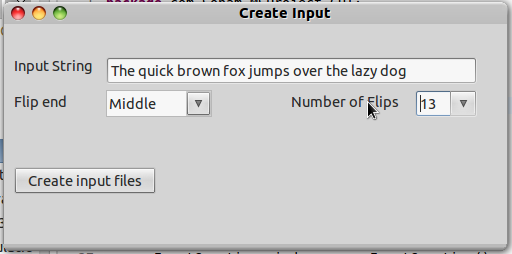
\includegraphics[width=5.2in]{inputcreationscreenshot.png}
  \end{center}
  \caption{Screen shot of GUI screen input, used to create the input files.}
  \label{fig:screenshotinputcreation}
\end{figure}

The click button on the GUI shown in figure 5.1 calls the createFile() function in class CreateInputFile, which 
is responsible for file creation. Details for both the class are shown in figure 5.2.

\begin{figure}
  \begin{center}
    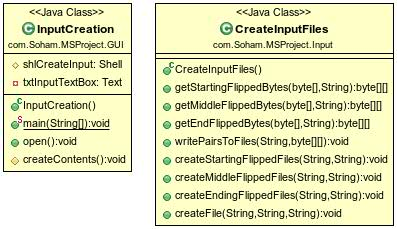
\includegraphics[width=4in]{Input.jpg}
  \end{center}
  \caption{Class diagram of the input creation.}
  \label{fig:UMLInputCreation}
\end{figure}

\subsection{Hash function implementation}

Each of the SHA-3 finalist hashing algorithm, were implemented in their own individual Java class. For the purpose
of the experiment, we only required the control over what input string went to the hashing algorithm, the number
of permutation rounds, and digest size in bits. Thus all the SHA-3 algorithms implement the interface "Hash" that
standardizes the call to each of finalist algorithm. The input string to the hash function, is the hexadecimal 
string representation of the ASCII bit value of the input string. The digest size is an integer from the following
four values 224, 256, 384 and 512. And the rounds can be anything between 1 and maximum number of rounds for a
given hash. For example in Keccak the number of rounds is 24, and if 25 is input in rounds, then the hashing will
be done for 24 rounds. So a safety check for a upward limit has not been built. By default, if you put zero, then
the recommended values of permutation rounds for the respective algorithm are used. The class diagram for the
SHA-3 hash function implementation is shown in figure 5.3.

\begin{figure}
  \begin{center}
    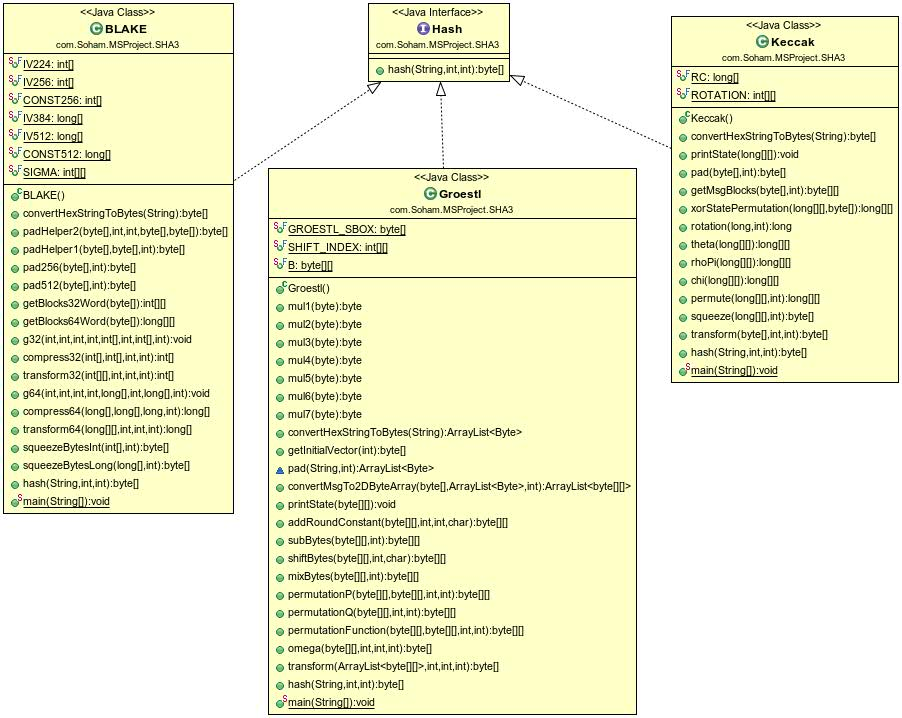
\includegraphics[width=6.8	in]{SHA3classes.jpg}
  \end{center}
  \caption{Class diagram of the classes for the 3 hash functions implemented.}
  \label{fig:UMLSHA3classes}
\end{figure}

\subsection{Experiment with different collision methods}

From the experiment selection dropdowns shown in figure 5.4, we can choose from the following factors
\begin{enumerate}
  \item The length of the chaining value that will be padded to the message, in bits.
  \item The algorithm for finding collision.
  \item The length of message digest in bits.
  \item The SHA-3 finalist algorithm, for hashing.
  \item Number of permuation rounds, for the hashing algorithm.
  \item The input case from start, middle or end, that you want to experiment with.
\end{enumerate}

\begin{figure}
  \begin{center}
    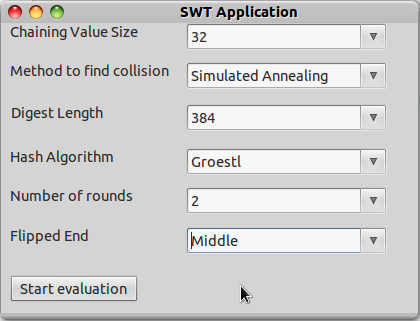
\includegraphics[width=4.25in]{experimentscreenshot.png}
  \end{center}
  \caption{Class diagram of the classes for the 3 hash functions implemented.}
  \label{fig:experimentscreenshot}
\end{figure}

The classes that instantiate the experiment, and their relation with the GUI class is shown in figure 5.5. It is 
the responsibility of the "Experiment" class, to go over the input files of the said category, and then provide 
the collision finding algorithms with the input message pairs, and instantiating them.

\begin{figure}
  \begin{center}
    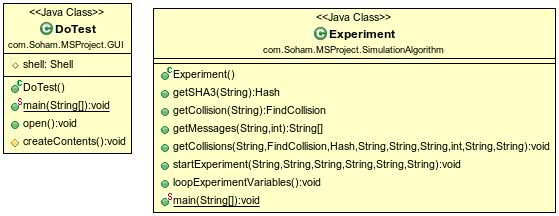
\includegraphics[width=5.65in]{ExperimentGUIClass.jpg}
  \end{center}
  \caption{Class diagram of the GUI class and the initiation of experiment.}
  \label{fig:UMLExperimentGUIClass}
\end{figure}

The Experiment class is the one that calls FindCollision algorithm, which is the parent class, that generates
the random chaining value as per the bit length provided. Evaluates the cost function, and generating neighbourhood
solution chaining values for the collision finding purpose. The relationship between the classes is shown in the
UML class diagram shown in figure 5.6.

\begin{figure}
  \begin{center}
    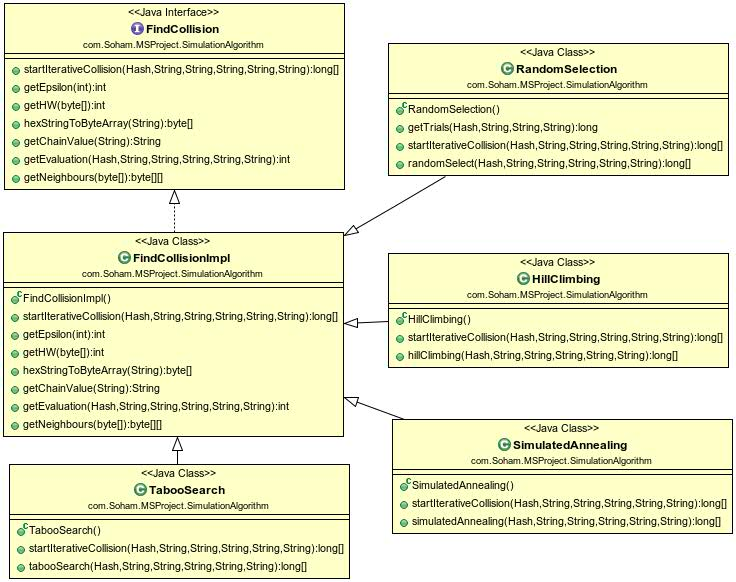
\includegraphics[width=7in]{FindCollisionClasses.jpg}
  \end{center}
  \caption{Class diagram of the classes for finding collisions.}
  \label{fig:UMLCollisionFindingClasses}
\end{figure}

\subsection{Testing the implemented code}

Code implementing hashing involves permuting and substituting large number of bits, resulting in subtle bugs to
magnify and distort the output results. As a consequence we have written, unit test cases to make sure, that our
code works in individual and parts, so that the correctness of the results can be guaranteed with absence of bugs
or bias in the code. InputTest class is created to make sure, that the toggling of the bits is done as expected.
ExperimentTest class makes sure, that the correct parameters are called and passed like the correct hashing
algorithm, with the expected digest size and rounds etc. The SHA3Test class makes sure that the implementation of 
all the SHA-3 finalist create the right message digests as expected. Finally the test class HillClimbTest makes
sure that neighbourhood test for the chaining value is done properly. The class diagram for the test is shown in
figure 5.7.

\begin{figure}
  \begin{center}
    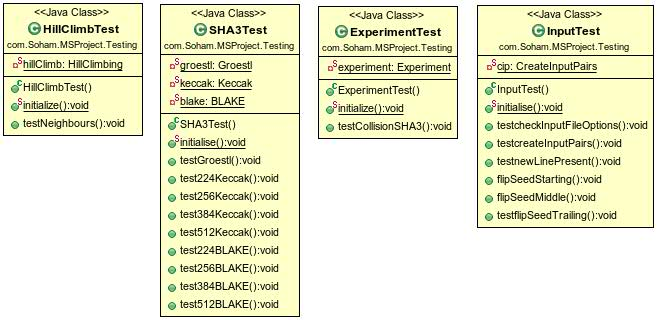
\includegraphics[width=6.75in]{testingcode.jpg}
  \end{center}
  \caption{Class diagram of the classes used for testing, using JUnit4.}
  \label{fig:UMLJUnitTestClasses}
\end{figure}
